
\section*{Materials and Methods}

Let  $\bm{b_{j}}$ represents the genetic effect of SNP-gene pair $j$ across $R$ = 44 tissues.

We assume the following mixture prior for the $R$ dimensional vector of true effects,  

 \begin{equation}
  \bm{b_{j}} | \bm{\pi},\bf{U}, \bm{\omega} \sim \sum_{k,l} \pi_{k,l} \;{\it N}_R(.; \bm{0}, \omega_l U_{k})
\end{equation}

Where ${\it N}_R(.; \bm{0}, \omega_l U_{k})$ denotes the density of a normal distribution with mean $\bm{0}$ and variance $\omega_l U_{k}$.


%As mentioned above, 
Each component of the mixture distribution is characterized by these prior covariance matrices, $U_{k}$ which capture the pattern of effects across tissues. Critically, this prior distribution is the same for all $J$ - hence the hierarchical incorporation of shared information.

\subsection{Covariance Matrices}\label{sssec:num1}

For a given $\omega_{l}$, we specify 4 `types' of $RxR$ prior covariance matrices $U_{k,l}$.
\begin{enumerate}

\item $U_{k=1,l}$ = $\omega_l$ $\mathbf{I}_{R}$

\item $U_{k=2,l}$ = $\omega_l$X_{z}$ The (naively) estimated tissue covariance matrix as estimated from the column-centered J \times R$ matrix of $Z$ statistics, $Z_{center}$: $\frac{1}{J}$ $Z_{center}$^{t}$ $Z_{center}$

\item $U_{k=3,l}$ = $\omega_l$ $\frac{1}{J}$ $V_{1...p}$ $d^{2}_{1...p}$   $V^{t}_{1..p}$ is the rank $p$ eigenvector approximation of the tissue covariance matrices, i.e., the sum of the first $p$ eigenvector approximations, where $\pcv_{1...p}$  represent the eigenvectors of the covariance matrix of tissues and $\pcd_{1...p}$ are the first $p$ eigenvalues.

\item $U_{k=4:4+Q-1,l}$ = $\frac{1}{J}(($\Lambda\mathbf{F})^{t} \Lambda \mathbf{F})_{q}$ corresponding to the $q_{th}$ sparse factor representation of the tissue covariance matrix %(not the sum of the first $q$, as above)

\item $U_{k=4+Q,l}$ = $\frac{1}{J}$ ($\($\Lambda \mathbf{F})^{t} \Lambda \mathbf{F}$ is the sparse factor representation of the tissue covariance matrix, estimated using all $q$ factors.



\item $U_{k=5+Q:R+4+Q,l}$ = $\frac{1}{J}$ $([1 0 0 . . ]'[1 0 0  . . .])$ %is the sparse factor representation of the tissue covariance matrix, estimated using all $q$ factors.
\item $U_{k=R+5+Q,l}$ = $\frac{1}{J}$ $([1 1 1 . . .]'[1 1 1 . . .])$
\item $[1 0 0 0 ...]$ or $[1 1 1  ...]$ represent configurations such that given membership,$\bm{b_{j}}$ arise from the same prior variance.
\end{itemize}

Critically, the computations above are estimated using the strongest snp per gene as characterized by the maximum absolute value across R tissues, in order to optimally initialize a `denoised' matrix of the true effects. 


\subsection{Deconvolution}
To retrieve a `denoised' or `deconvoluted' estimate of the non-single rank dimensional reduction matrices, we then perform deconvolution after initializing the EM algorithm with  the matrices specified in (2), (3) and (5). The final results of this iterative procedure preserves the rank of the initialization matrix, and allows us to use the `true' effect at each component component $\bm{{b}_{j}}$ as missing data in deconvoluting the prior covariance matrices. In brief, this algorithm works by treating not only the component identity but also the true effect $\bm{{b}_{j}}$  as unobserved data, and maximizing the likelihood over the expectation of the complete data likelihood, considering the values $\bm{{b}_{j}}$ as extra missing data (in addition to the indicator variables $q_{ij}$) (Bovy et al, 2014). 
%%
%This allows us to write down the `full data' log likelihood as follows:
%
%\begin{equation}
%\begin{center}
%\begin{aligned}
%\phi=\sum_{J} \sum_{K} q_{jk} ln \alpha_{k} \it{N}(\hat{\bm{b}}_{j}|0,U_{k}+V_{j})\\
%\phi=\sum_{J} \sum_{K} q_{jk} ln \alpha_{k} \it{N}(\bm{{b}_{j}}|0,U_{k})
%\end{aligned}
%\end{center}
%\end{equation}
%
%
%Where $\alpha_{k}$ represents $\pi_k$ and $q_{jk}$ is the latent identifier variable.
%
%Now at the E step:
%
%\begin{equation}
%\begin{center}
%\begin{aligned}
%q_{jk}= \alpha_{k} \it{N}(\hat{\bm{b}}_{j};0,U_{k}+V_{j})\\
%b_{jk}= E(b_{jk} | \hat{\bm{b}}_{j};0,U_{k}+V_{j})\\
%B_{jk}=E(U_{jk} | \hat{\bm{b}}_{j};0,U_{k}+V_{j})
%\end{aligned}
%\end{center}
%\end{equation}
%
%
%\begin{equation}
%\begin{center}
%\begin{aligned}
% \alpha_{k} = \frac{1}{J} \sum_{J}  q_{jk} \\
%U_{k}= \frac{1}{q_{k}}\sum_{J} q_{jk} b_{jk} b_{jk} + B_{jk}
%\end{aligned}
%\end{center}
%\end{equation}
%
%
%
%%
%%\subsection{Generation of List of Covariance Matrices}
%%
%%We then use these three non single-rank covariance matrix in place of our original choice of the empirical covariance matrix, SFA and SVD approximations. Here, I also used the Identity (K=1), 5 single-rank SFA factors (K=4-9), and the 44+1 $eqtlbma.lite$ configurations (K=10:54) in steps (7) and (8) to a assemble a full list of covariance matrices. Briefly, these  $eqtlbma.lite$ are an attempt to capture 'singleton' and 'fully shared' configurations in which the gene-snp pair is active in only one or all tissues. In the latter case, the variance of the distribution of underlying effect sizes is equal in all tissues.  This is 54 matrices, and we then proceed to chooses an $'L'$ element grid according to the range of effect sizes present in the overall data set in order to create a KxL list of covariance matrices. In the GTeX data set described in the text, we choose a grid with 22 $\omega$ for a total of 1188 covariance matrices.

Let us concatenate the list of all KxL combinations of prior covariance matrices $U_{k}$ and their scaling parameters $\omega_{l}$ into a KxL list and assign this length $P$ for simplicity of notation.

Now each $U_{p}$ imparts information about both $\emph{scale}$ and $\emph{direction}$.


\subsection{Likelihood}

By maximum likelihood in each tissue separately, we can easily obtain the observed estimates of the standardized genotype effect sizes, $\hat{\bm{b}}_{j}$, and their observed squared standard errors recorded on the diagonal of an $R \times R$ matrix denoted $\hat{V}_{j} = \Var(\hat{\bm{b}}_{j})$. 
We assume that the matrix of standard errors of $\hat{\bm{b}}_{j}$, $V_{j}$ as approximated by $\hat{V_{j}}$ is diagonal and  that $\hat{V}_{j}$ is an accurate point estimate for the standard error and that these standard errors are independent between tissues.

If we now view $\hat{\bm{b}}_{j}$ and $\hat{V}_{j}$ as \emph{observed data}, we can write a new ``likelihood'' using only the sufficient statistics,   $\hat{\bm{b}}_{j}$ and $\hat{V}_{j}$:

\begin{equation}
\hat{\bm{b}}_{j} | \bm{b}_{j}, \hat{V_{j}} \sim {\it N}_R(\hat{\bm{b}}_{j}; \bm{b}_{j}, \hat{V}_{j})
%&= \sum_{p}^{P} \pi_{p} {\it N}_R(\hat{\bm{b}}; \bm{0}, U_{p} + V_{j})
\label{eqn:new_lik}
\end{equation}

In brief, though we report the analysis using $\hat{\bm{b}}_{j}$ and its standard error, inference can be similarly performed using the vector of observed Z statistics ${Z}_{j}$ with the matrix of squared Standard Error $\hat{V}_{j}$ thus defined as the RxR Identity Matrix. This is deemed the `EZ' model and assumes exchangeable standardized effects, e.g., that effects tend to scale with their standard error:

 \begin{equation}
  \frac{\bm{b_{j}}}{\bm{\hat{s_{j}}}} | \bm{\pi},\bf{U}, \bm{\omega} \sim \sum_{k,l} \pi_{k,l} \;{\it N}_R(.; \bm{0}, \omega_l U_{k})
\end{equation}

Likelihood based methods can then used to determine the superior model fit (see Supplement (Testing/Training) for details).

\subsection{Mixture Weights: Estimate $\hat{\bm{\pi}}$}\label{sssec:ebweights}
We wish to choose the model which best maximizes the probability of observing the data set. First, we must estimate the prior mixture weights $\pi$ by maximizing the likelihood 

\begin{equation}
\begin{aligned}
L(\pi;\hat{\bm{b}}, \bm{s}) &= p(\hat{\bm{b}} | \bm{s},\pi) \\
&= \prod_{j=1}^J \sum_{p}^{P} \pi_{p} P(\hat{\bm{b}}_{j} | \hat{\bm{s}}_{j}, z_{j}=p)\\
&= \prod_{j=1}^J \sum_{p}^{P} \pi_{p} {\it N}_R(\hat{\bm{b}}; \bm{0}, U_{p} + V_{j})
\label{eq:cdll}
\end{aligned}
\end{equation}



Here, in order to obtain mixture weights $\bm{\pi}$ which reflect the abundance of each pattern of sharing in the overall data set, we use a random set of gene-snp pairs (i.e., not restricting our analysis to the pairs with the strongest Z statistics used in the section above) and obtain the maximum likelihood estimates of the mixture weights, $\hat{\bm{\pi}}$, which maximize the complete data likelihood ($\ref{eq:cdll}$) (Laird 1977; Barut 2005).

\begin{itemize}
\item  To estimate the hierarchical prior weights $\hat{\bm{\pi}}$ we compute the likelihood at each of these randomly chosen gene-snp pairs $j$ by evaluating the probability of observing $\bm{\hat{b}_{j}}$ given that we know the true $\bm{b_{j}}$ arises from component $\textbf{p}$ (see \ref{eqn:new_lik}).
\item  Use the Expectation Maximization (EM) algorithm to estimate the optimal combination of weights as $\bm{\hat{\pi}}$ using the  $\textbf{JxP}$ matrix of likelihoods computed according to ($\ref{eqn:new_lik}$).
\end{itemize}

%We then use these weights to estimate the test set log-likelihood.

\subsection{Posterior Quantities}\label{sssec:posteriors}

Armed with the prior mixture weights stored in the $P$ vector $\hat{\bm{\pi}}$ we proceed to the inference step and compute the posterior weights ($\ref{eqn:postpi}$) and corresponding posterior quantities across all original 16,069 gene-snp pairs. %In brief, the posterior mean and tissue specific tail probabilities are computed across all K components for each gene snp pair, and then weighted according to the posterior weights. This is performed in the $\textbf{weightedquants}$ step.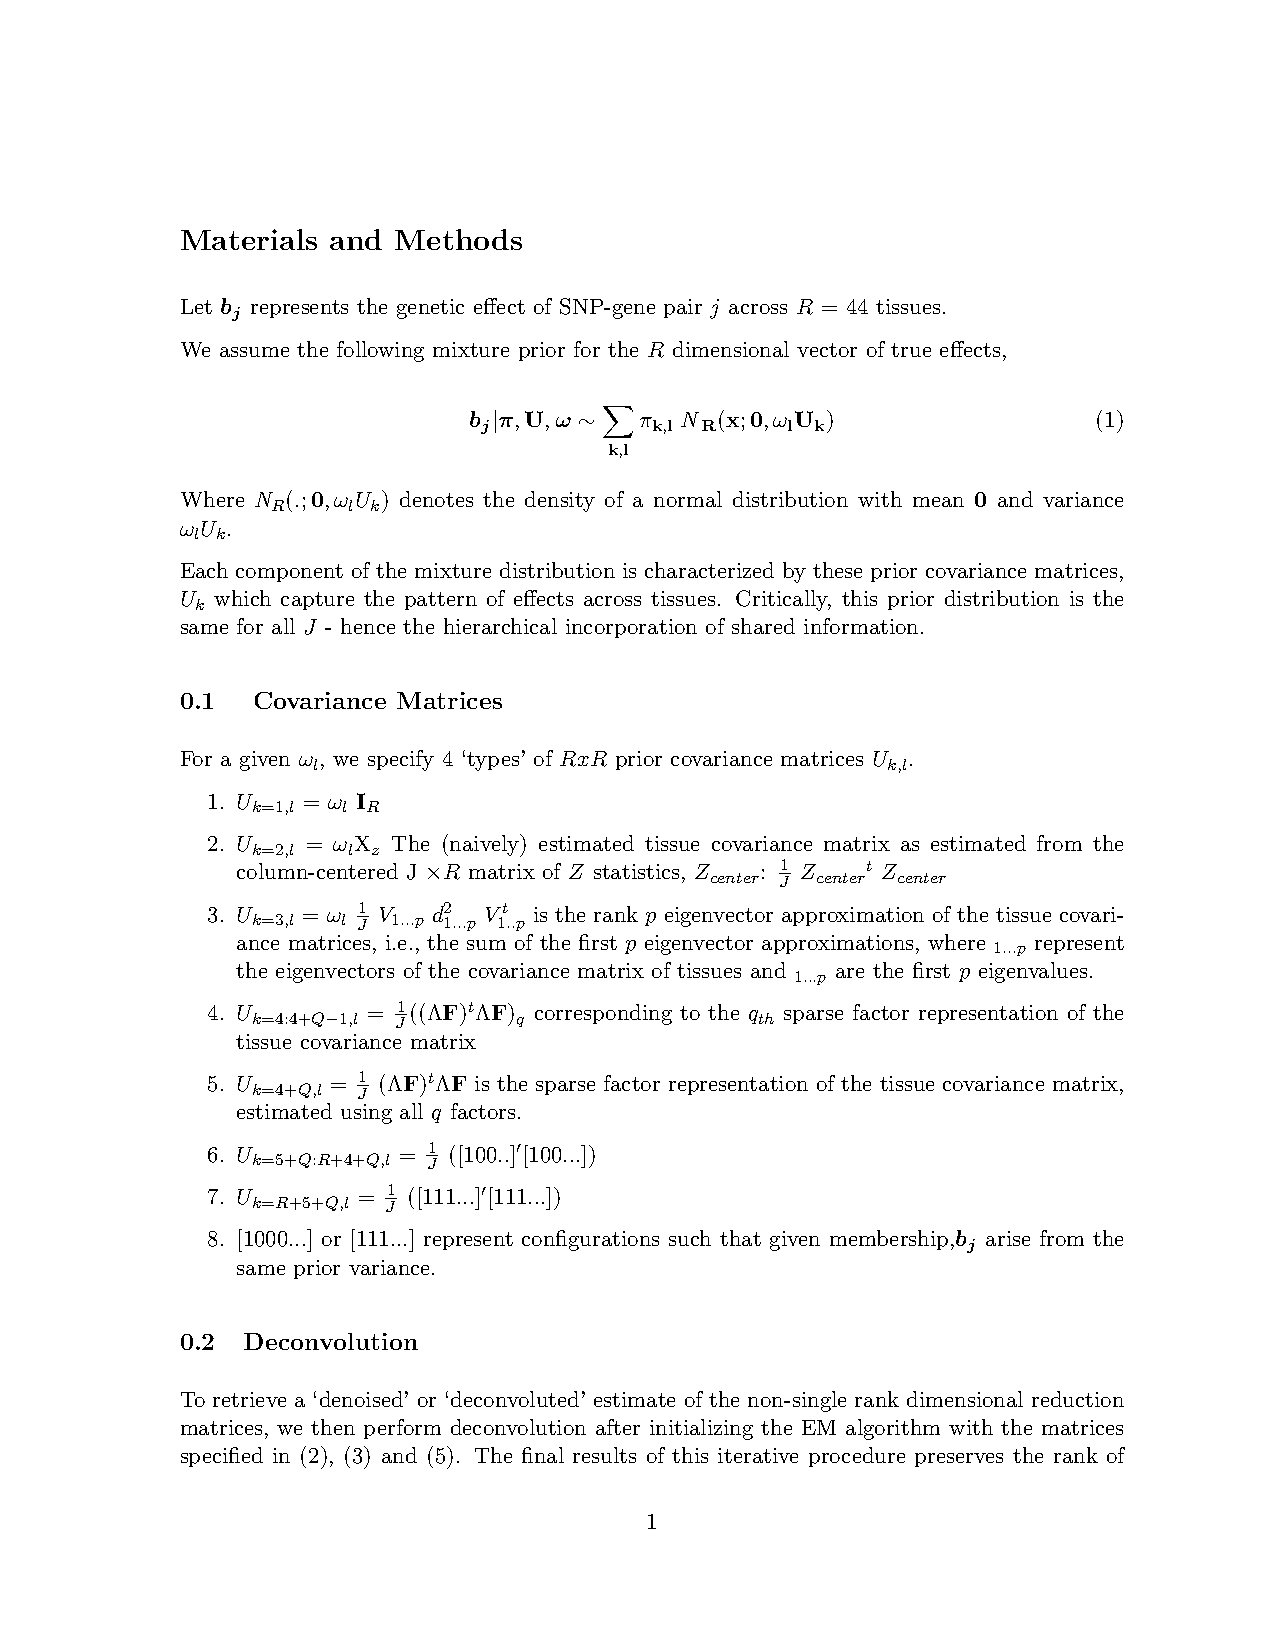
\includegraphics[]{Methods.pdf}

We aim to report posterior quantities for a given gene-snp pair $\textbf{j}$. We know that for a single multivariate {\it Normal}  the posterior on  $\bm{b} | U$ is  simply: 

\begin{equation}
\[
\bm{b} | \hat{\bm{b}} \sim {\it N}_R(\bm{\tilde{\mu}}, \tilde{U})
\]
\end{equation}

where:
\begin{itemize}
\item $\bm{\tilde{\mu}}= \tilde{U}(\hat{V}^{-1} \hat{\bm{b}})$
\item $ \tilde{U} = ({U}^{-1} + \hat{V}^{-1})^{-1}$.
\end{itemize}


Furthermore, a mixture-multivariate normal prior and a normal likelihood yields a mixture multivariate posterior, where the final posterior distribution is simply a weighted combination of multivariate normal distributions, where for each gene-snp pair $\textbf{j}$ is now characterized by it's posterior mean $\tilde{\bm{\mu}}_{jp}$ and covariance  $\tilde{U}_{jp} = (U_{p}^{-1} + \hat{V}_{j}^{-1})^{-1}$.

\begin{equation}
\begin{aligned}
  \label{eq:mixpost}
\bm{b}_{j} | \hat{\bm{b}}_{j}, \hat{V}_{j}, \hat{\bm{\pi}} 
%&= \sum_{k=1,l=1}^{K,L} \sim {\it N}_R(\bm{\mu}_{1kl}, U_{1kl})%p(\bm{b}_{j} | \hat{\bm{b}}_{j}, \hat{V}_{j}, z_{j}=k,l) 
%p(z=k,l | \hat{\bm{b}}, \hat{V}, \hat{\bm{\pi} }),%v_{j}=1)
 %\\
\sim \sum_{p}^{P}  \tilde \pi_{jp} {\it N}_R (.;\bm{\tilde{\mu}}_{jp},\tilde{U} _{jp} )%,v_{j}=1) 


\end{aligned}
\end{equation}

Where ${\it N}_R(.; \bm{\tilde{\mu}}_{p}, \tilde{U} _{p})$ denotes the density of a normal distribution with mean $\bm{\tilde{\mu}}_{p}$ and variance $\tilde{U} _{p}$ and the posterior mixture weight $\tilde \pi_{p}$ is simply:

\begin{equation}
\tilde \pi_{jp} =\frac{ p(\hat{\bm{b}}_{j}| \hat{V}_{j}, z_{j}=p) \hat \pi_{p} } {\sum_{p=1}^{P} p(\hat{\bm{b}}_{j}| \hat{V}_{j}, z_{j}=p) \hat\pi_{p}}
 \label{eqn:postpi}
\end{equation}

Where $z_{j}=p$ is the latent variable indicator of the component identity and each $\hat\pi_{p}$ represents the Maximum Likelihood Estimate of the prior mixture weights assigned to each component according to (\ref{eq:cdll}).

\subsection{Reported Quantities}

For every gene-snp pair `j', we aim to report the effect size as the posterior mean, defined as:

\begin{equation}
\begin{aligned}
E(\bm{b}_{j} | \hat{\bm{b}}_{j}, \hat{V}_{j}, \hat{\bm{\pi}})
%&= \sum_{k=1,l=1}^{K,L} \sim {\it N}_R(\bm{\mu}_{1kl}, U_{1kl})%p(\bm{b}_{j} | \hat{\bm{b}}_{j}, \hat{V}_{j}, z_{j}=k,l) 
%p(z=k,l | \hat{\bm{b}}, \hat{V}, \hat{\bm{\pi} }),%v_{j}=1)
 %\\
= \sum_{p}^{P}  \tilde \pi_{p} \bm{\tilde{\mu}}_{p} %,v_{j}=1) 
\end{aligned}
\label{eq:mixmean}
\end{equation}


And the local false sign rate, or posterior probability of incorrectly identifying the sign of the effect for a given tissues `r' as :

\begin{equation}
  \label{eq:lfsr}
\begin{split}
P(b_{jr})= 1-max[{\sum_{p}}p({b_{j,r}}>0|\hat{\bm{b}}_{j}, \hat{V}_{j}, z_{j}=p)\tilde \pi_{p}, {\sum_{p}}p({b_{j,r}}<0|\hat{\bm{b}}_{j}, \hat{V}_{j}, z_{j}=p)\tilde \pi_{jp}]
\end{split}
\end{equation}

For the results section of this paper, we report the  posterior mean ($\ref{eq:mixmean}$) and LFSR ($\ref{eq:lfsr}$) for the `top' snp per gene, but armed with the hierarchical weights computed in (\ref{eq:cdll}) and covariance matrices $\textbf{U}$ the posteriors can be computed for any gene-snp pair.

\subsection{Simulation Framework}\label{sssec:simulation}


In brief:
\begin{enumerate}
\item Assemble a list of simulation covariance matrices reflecting the GTEX `patterns' $\bm{U}$ from the 8 $U_{k}$ `learned' from the GTEX data-set as items (2) through (5) (see Methods \ref{sssec:num1} for details)  scaled by the maximum value along the diagonal, such that the maximal value along the diagonal of all 8 $U_{k}$ is 1.
\item For `true effects', here 400 simulated gene-SNP pairs, choose a true-component identity $\bm{z}_{j}=k$ by sampling with replacement from one of eight possible patterns $U_{k}$ 
\item To simulate a variety of effects sizes along each pattern of covariance, for each of these true effect vectors $\bm{b}_{j}$, $\omega_{j}$ is the absolute value of  the random variable $x \sim {\it N}(\bf{x}; \bm{0}, 1)$.
\item $ \bm{b}_{j}  | \bf{U}, \bm{\omega}, \bm{z} \sim{\it N}_{44} (.; \bm{0}, \omega_j U_{k})$. Here, ${\it N}_R(.; \bm{0}, \omega_j U_{k})$ denotes the density of a normal distribution with mean $\bm{0}$ and variance $\omega_j U_{k}$ .

%\item For all 50,000 gene snp pairs: Treating $V_{j}$ as known, simulate an R vector of Standard Errors S_{j} ${\it N} (.; \bm{0.11}, 0.001))$ in order to emulate  the observed scenario in which the errors are known and IID. $V_{j}$ is diagonalized $S_{j} ^2$.
\item For all 50,000 gene snp pairs, treat $\bm{s}_{j}$ as known R-vector of standard error, we simulate the R vector of $Error$ as $\textbf{E}_{j} \sim {\it N} (.; \bm{0}, V_{j} )$ where $V_{j} $ represents the diagonalized matrix of squared known standard error, $\bm{s}_{j}^{2}$. 
\item For all 50,000 gene snp pairs, $\hat{\bm{b}}_{j} | \bm{b}_{j} , V_{j} = \bm{b}_{j} + \textbf{E}_{j}$ %\ \sim \Norm_R(\bf{x}; \bm{b}_{j}, {V}_{j}) 
and the observed Z statistic for each gene-snp-tissue coordinate can be obtained from this vector of estimated $\hat{\bm{b}}_{j}$ and (known) standard error, $\textbf{s}_{j}$ as $\frac{\hat{\bm{b}}_{j}}{\bm{s_{j}}}$.
\item In the tissue-specific scenario, for $35\%$ of the `true' gene SNP pairs, simulate $\bm{b}_{j}$ according to one of `5' tissue-specific configurations, using the effect sizes obtained from the simulated $\omega_{j}$ above, according to the sparse matrix described in item (6) (Methods \ref{sssec:num1}). 
\item Following the framework (detailed Method \ref {sssec:posteriors}) perform inference on the observed summary statistics $\hat{\bm{b}}_{j}$ to estimate the $\emph{posterior mean}$ ($\ref{eq:mixmean}$) and $\emph{lfsr}$ ($\ref{eq:lfsr}$) for all 50,000 gene-snp pairs. 
\end{enumerate}


\section*{Supporting Information}

\subsection{Testing and Training}

In order to determine the optimal number and rank of the covariance matrices, we divide our data set into a training and test data set, each containing 8000 genes.

In the training set, we proceed as above: choosing the top SNP for each of the 8000 genes, creating a list of covariance matrices through deconvolution and grid selection of these top 'training gene-snp' pairs. 

Then, within the training data, we similarly choose a random set of gene-snp pairs (restricting our analysis to genes contained in the training set). Specifically, we choose 20,000 random-gene snp pairs and use the EM algorithm to learn the mixture proportions $\bm{\hat{\pi}}$  from this data set as in (\ref{eq:cdll}).

We then use the KxL vector of $\pi$ from the training set to estimate the log likelihood of each data point in the test data set. If our model is biased (or `overfit') to the training data set, then a larger number of covariance matrices may actually decrease the test log-likelihood. 

\subsection{Visualizing All Patterns of Sharing}
\begin{figure}[htbp]
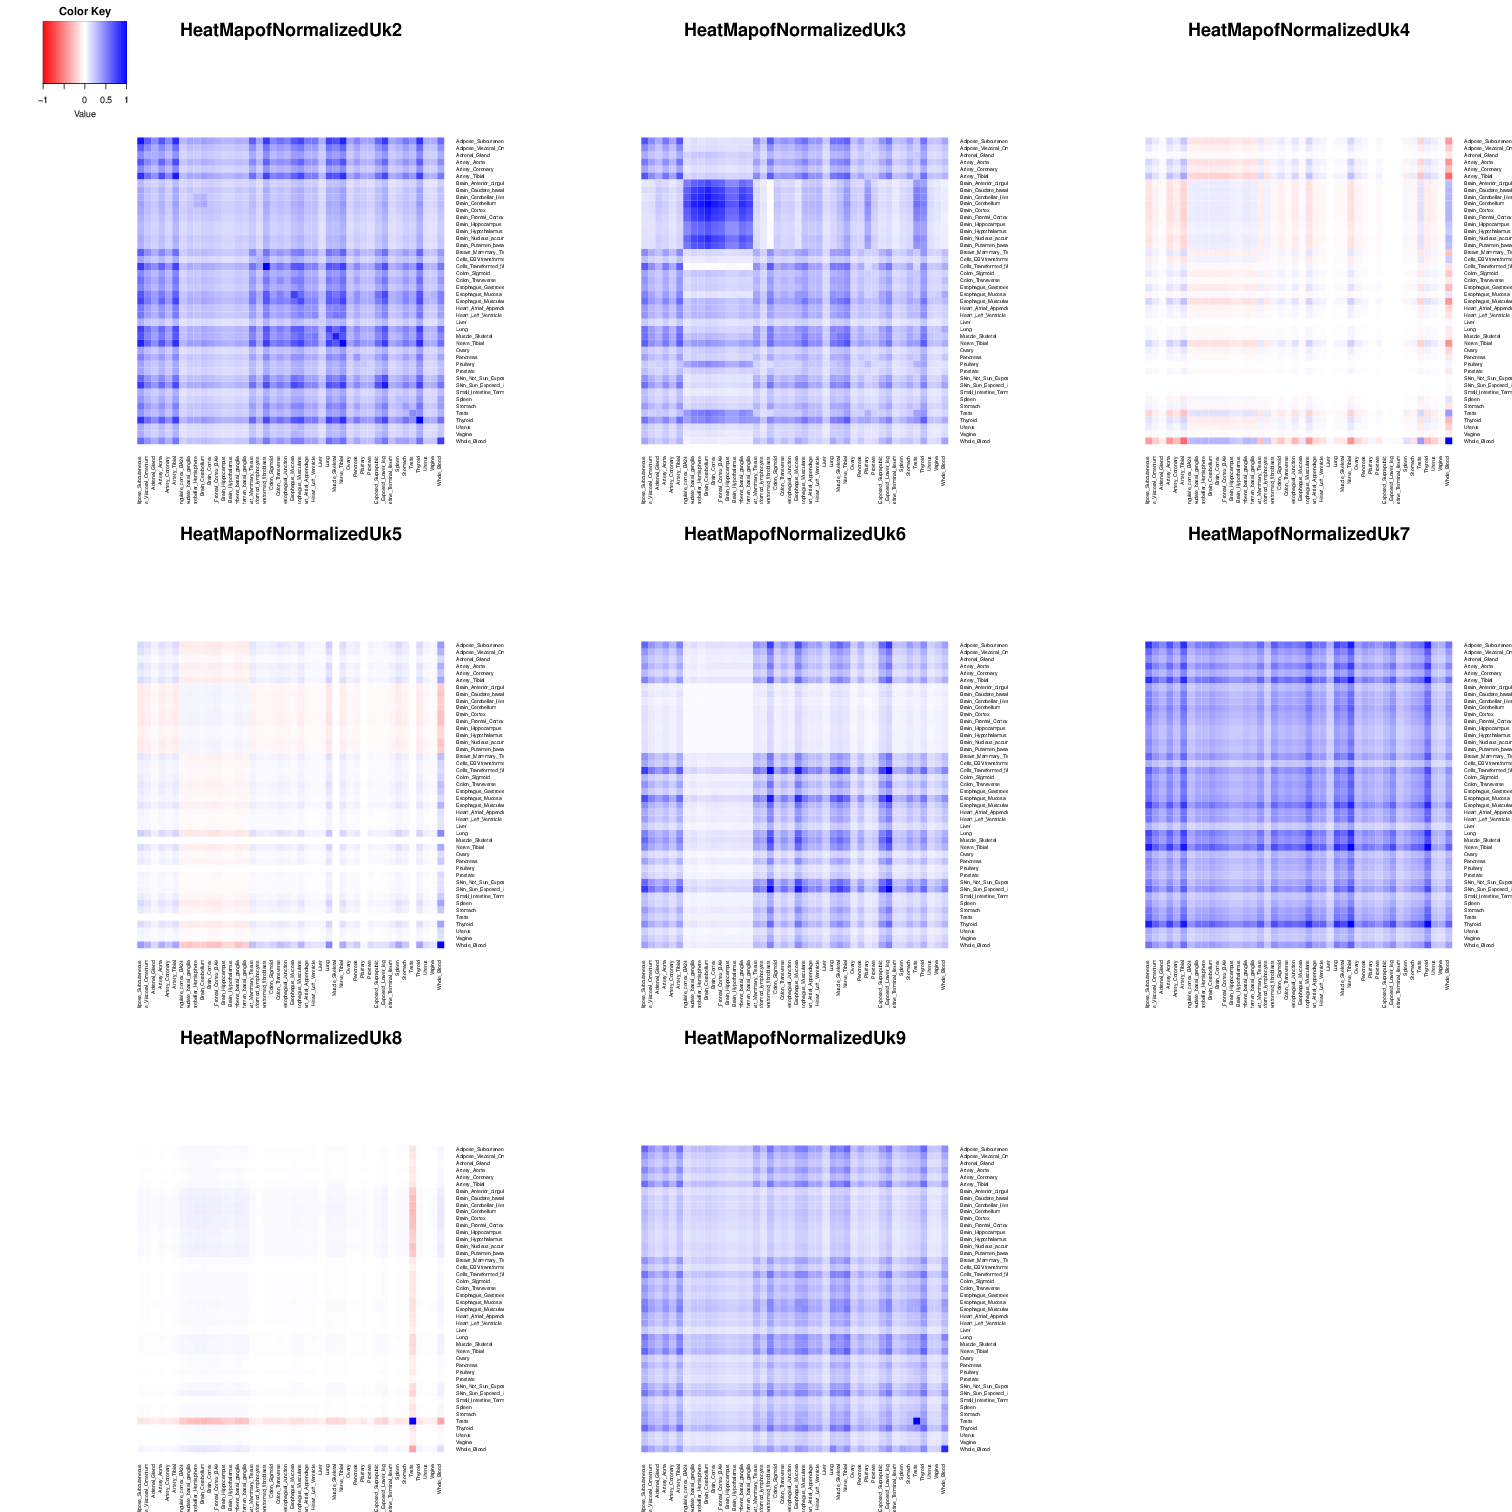
\includegraphics[width=10cm]{Figures/gtexresultcompiledheatmaps.png}
\caption{\textbf {Diverse Array of Relationships among tissues.} Here, we use heatmaps to visualize all the patterns of sharing present in the data}
\label{fig:allheat}
\end{figure}\newline

%In this data set, we find that K=1188 set of covariance matrices containing the Identity, the denoised empirical covariance matrix, rank five SFA approximation and rank 3 SVD approximation as well as 5 single-rank SFA factors and the 45 $eqtl.bma.lite$ configurations maximized this likelihood.

